\section{Research Methodology}
This chapter describes the research methodology used in this thesis. The work follows the Design Science Research Methodology (DSRM) framework as described by~\citet{DSRMethodology2007}. DSRM was selected because the thesis involves both the creation of a software artifact and the evaluation of its performance in a real-world environment which aligns well with the design science approach. The artifact itself was comissioned by an employer with specific requirements for improving the communication capabilities of their existing systems, therefore a practical need was driving the design decisions alongside the research objectives.
\subsection{Design Science Research Methodology}
Design science research is concerned with creating and evaluating IT artifacts that are intended to solve identified problems~\citep{DSRMethodology2007}. It differs from other research frameworks by not only trying to understand reality but also attempting to create something that serves a purpose. The DSRM framework provides a process model for conducting this type of research consisting of six activities: problem identification and motivation, definition of the objectives for a solution, design and development, demonstration, evaluation and communication.

\begin{figure}[ht]
    \centering
    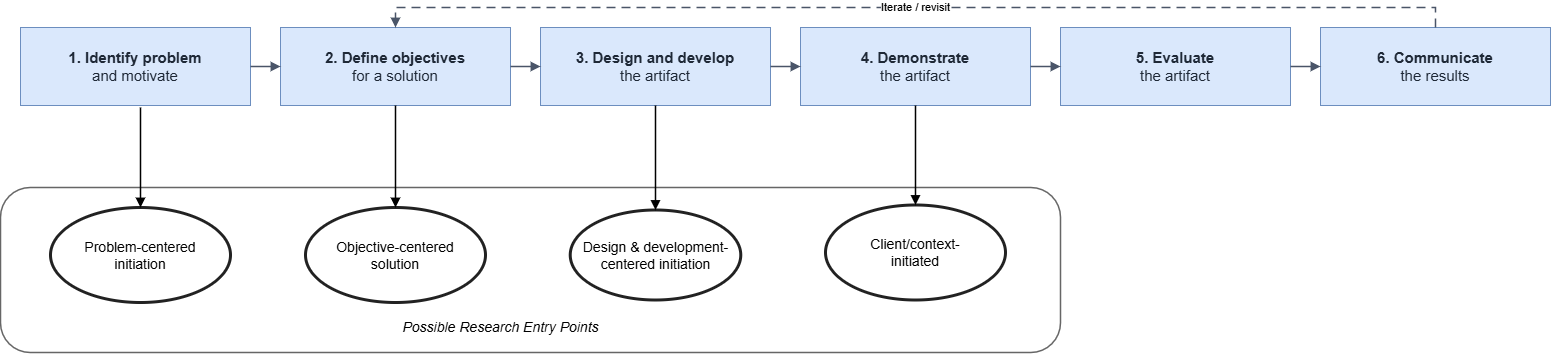
\includegraphics[width=1.0\textwidth]{figs/dsrm_process.png}
    % TODO: Insert DSRM process model diagram
    \caption{DSRM process model as presented by~\citet{DSRMethodology2007}. The process includes six activities and four possible entry points depending on how the research is initiated.}
    \label{fig:dsrm-process}
\end{figure}
The framework allows for different entry points into the process depending on how the research is initiated~\citep{DSRMethodology2007}. The problem-centered approach starts from activity 1 when the idea comes from observing a real problem. An objective-centered solution starts from activity 2 when there is an industry or research need that can be addressed by developing an artifact. A design and development-centered approach starts from activity 3 when an artifact already exists or is being built before formalizing the research questions around it. The research proccess begins from the activity associated with the initiator, whereas other activities can be optionally excluded if they pose no relevancy to the research. 
\par
In this thesis all three entry points are relevant to some extent. The primary motivation is design and development-centered, because the artifact was originally developed as part of employment at Observis Oy. A practical need for improved CBRN communication capabilities over satellite networks arose from customers' requirements. Combined access to existing domain knowledge codebases and testing infrastructure shaped what could realistically be built and evaluated.
\par
At the same time there is also a problem-centered motivation behind this work. CBRN defense teams operate in environments where terrestrial communication infrastructure may be unavailable, damaged or deliberately disrupted as discussed in Chapter 1. The limitations of traditional transport protocols like TCP over high-latency lossy satellite links are well documented in literature~\citep{LangleyAdam2017TQTP}, resulting in a clearly identifiable problem that needs solving.

Furthermore, an objective-centered perspective is also applicable because new technologies, such as commercial LEO satellite internet (Starlink) and modern transport protocols (QUIC) have emerged recently, making it possible to achieve better latency and coverage than what was previously feasible with older technology combinations~\citep{Benghe2026}. These technological developments created new possibilities that did not exist before, therefore defining objectives around them became meaningful.

This work is at the intersection between industrial practice and academic research, which is reflected by the relevance of the three entry points.  This hybrid approach is consistent with how DSRM has been applied across different fields where multiple motivators often coexist within same project~\citep{DSRMethodology2007}.

\subsection{Research Process}

The DSRM framework is followed throughout this thesis by mapping each activity to corresponding chapters:

\begin{itemize}
    \item \textbf{Activity 1 --- Problem Identification and Motivation:} Addressed in Chapter~1 where CBRN defense field, LEO satellite networksand QUIC protocol are introduced alongside motivation, context, objectives and scope delimitations.
    
    \item \textbf{Activity 2 --- Objectives for a Solution:} Defined through research questions RQ1 and RQ2, hypotheses H1 and H2, together with concrete objectives O1-O4 outlined in Chapter~1. These objectives describe what a successful outcome looks like.
    
    \item \textbf{Activity 3 --- Design and Development:} Covered in Chapter~tbd, describing system architecture protocol design, implementation details and limitations simplifications made during development.
    
    \item \textbf{Activity 4 --- Demonstration:} Conducted through field measurements over Starlink network using TCP baseline, QUIC implementation and QUIC+ML variant  with results presented in Chapter~tbd.
    
    \item \textbf{Activity 5 --- Evaluation:} Analysis comparing observed results against defined metrics hypotheses, leading to discussion of findings and validity threats in Chapter~tbd .
    
    \item \textbf{Activity 6 --- Communication:} This thesis itself serves as the primary means for the communication of findings to academic audience and field professionals.
\end{itemize}

A central theme throughout this work is that new technology emerges faster than traditional communication protocols can adapt to changing conditions. This particularly applies to satellite environments, where latency and handovers packet loss vary significantly, depending on location, weather and constellation state. Instead of designing completely new protocols from scratch, this approach investigates whether combining existing technologies such as QUIC and LEO satellite internet can provide acceptable performance for CBRN use cases without requiring modifications of underlying network infrastructure. The theoretical background gathered in Chapter~2 establishes necessary context for understanding why these particular technologies were selected and how they interact with each other.
\par
The evaluation metrics defined later in Chapter~tbd reflect what can be practically measured, given the constraints of real-world testing over commercial satellite link. Lower latency is generally considered better, but cannot be measured in isolation as throughput, jitter, processing overhead and recovery time after handover events must be considered together to form a complete picture of transport performance.
\subsection{Evaluation Metrics}
% the artifact should exist first, then it will become apparent what can be measured and what statistical methods can be used to proccess the data
% in simple terms, lower latency = better, but that can't be measured in a vacuum, there's throughput, jitter, proccessing penalties, rare anomaly events etc to consider
\subsection{Experimental Design}
% the hardware and software involved, how the system/artifact was created
% how it can be reproduced I suppose, why measuring it was / wasn't accurate
\clearpage


